\par Cell detection and characterization are important for applications in medical diagnosis and food safety \cite{mansor}. With the advent of micro-electro-mechanical systems (MEMS), cell characterization techniques have developed with increasing precision and cost-effectiveness. One of these techniques is impedance spectroscopy. Cell impedance spectroscopy measures the electrical impedance of cell(s) over a range of frequencies and can identify cell types, differentiate cell states, and provide information about cell components. With significantly increased manufacturing precision provided by MEMS technologies, cell impedance spectroscopy has been miniaturized to measure the impedance spectrum of single cells instead of macro suspensions. 

\par The applications of single cell impedance spectroscopy are extensive. In medical diagnostics, the ability to isolate the impedance spectrum of a single cell allows the diagnosis of diseases with very small limits of detection, such as early detection of cancer by identifying circulating tumor cells that can be as scarce as 1 cell per mL of blood \cite{mansor-1}. In food safety single cell spectroscopy can detect pathogens in a rapid and inexpensive manner, such as E.Coli and Salmonella contamination in water sources \cite{mansor-3}. In addition, impedance spectroscopy is an important tool in research, with the ability to quickly measure a cell's state and response to stimuli. 

\par The focus of this thesis will be to reevaluate and optimize the Cal Poly Biofluidic lab's single cell impedance sensor.

\section[Cal Poly's IS System]{The Cal Poly Biofluidic Lab's Cell Impedance System}

\par In 2009, Josh Fadriquela and Stephanie Hernandez created a cell impedance spectroscope system for the Cal Poly biofluidic lab under the direction of Dr. Clague \cite{fadriquela_design_2009-1,hernandez_single_2009-1}. The purpose of the project was to create a system to measure single cell impedance measurements. The project included the design of the electrodes and microfluidic channels of the impedance sensor, manufacturing of the device, installment of requisite hardware, and development of software necessary for impedance measurements. 

\begin{figure}[h]
    \centering
    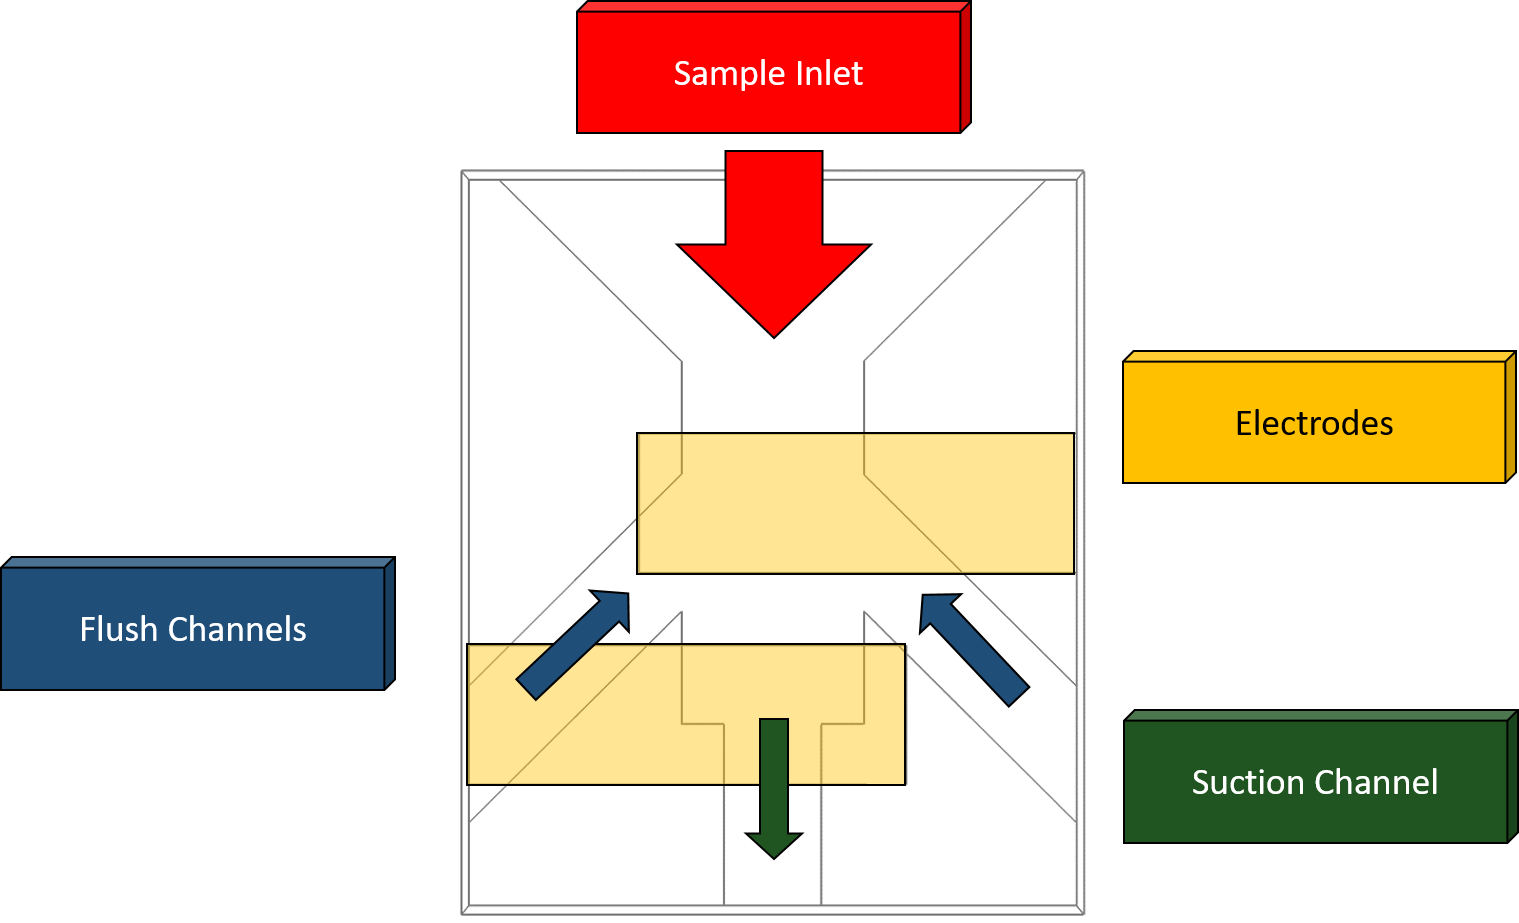
\includegraphics[width=\textwidth]{images/josh_steph_design.png}
    \caption{Functional diagram of cell impedance sensor chamber.}
    \label{fig:josh-steph_functional_diagram}
\end{figure}

\par The impedance sensor was designed with two 11.5 micron wide electrodes with a 5 micron gap that lays under a 15 by 15 micron target measurement area. The device isolates a cell by activating flush and suction channels once a cell from the sample inlet wanders into the test chamber with the purpose of keeping the cell in the test chamber and other cells out (figure \ref{fig:josh-steph_functional_diagram}). Once the device captures a cell, voltage signals over a range of frequencies are applied 

\begin{figure}[h]
    \centering
    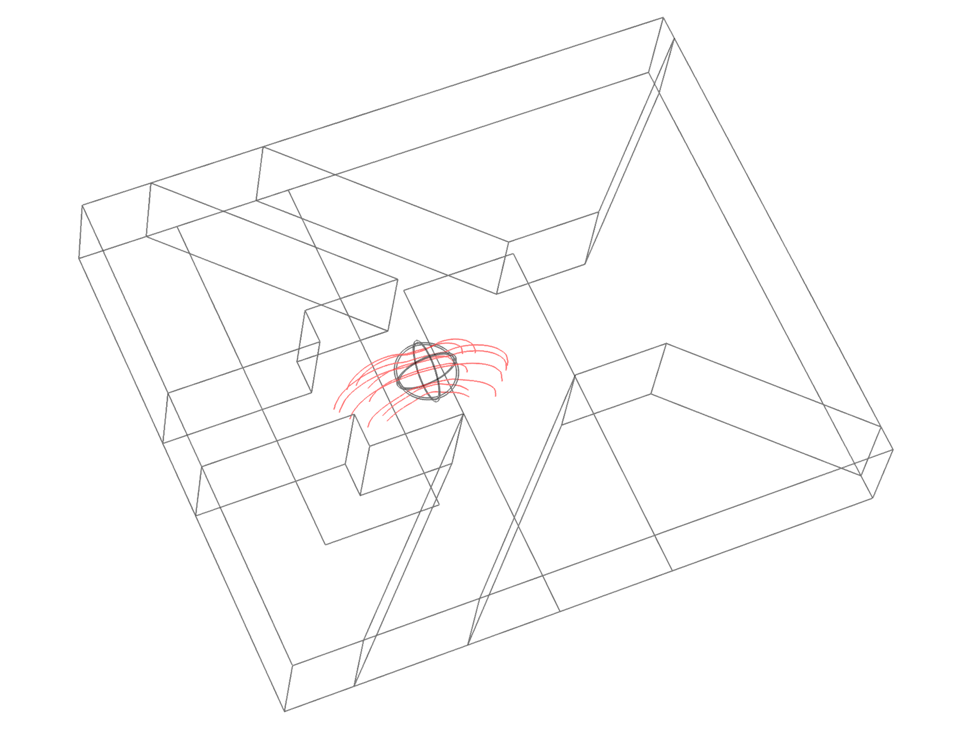
\includegraphics[width=0.9\textwidth]{images/josh_steph_sim.png}
    \caption{Example of desired device behaviour using a COMSOL simulation of electric field lines through a cell. A detailed description of the COMSOL model is presented in section \ref{}}
    \label{fig:josh-steph_sim}
\end{figure}


\begin{figure}[h]
    \centering
    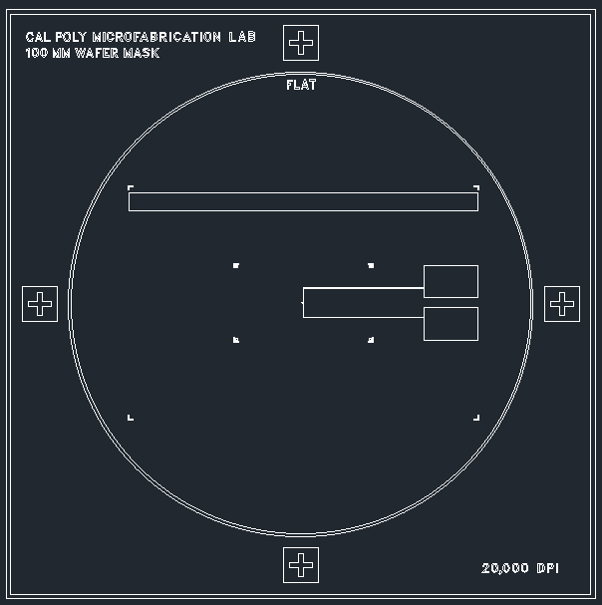
\includegraphics[width=0.6\textwidth]{images/electrode_mask.png}
    \caption{Electrode mask by Stephanie Hernandez \cite{hernandez_single_2009-1}}
    \label{fig:electrode_mask}
\end{figure}

\begin{figure}[h]
    \centering
    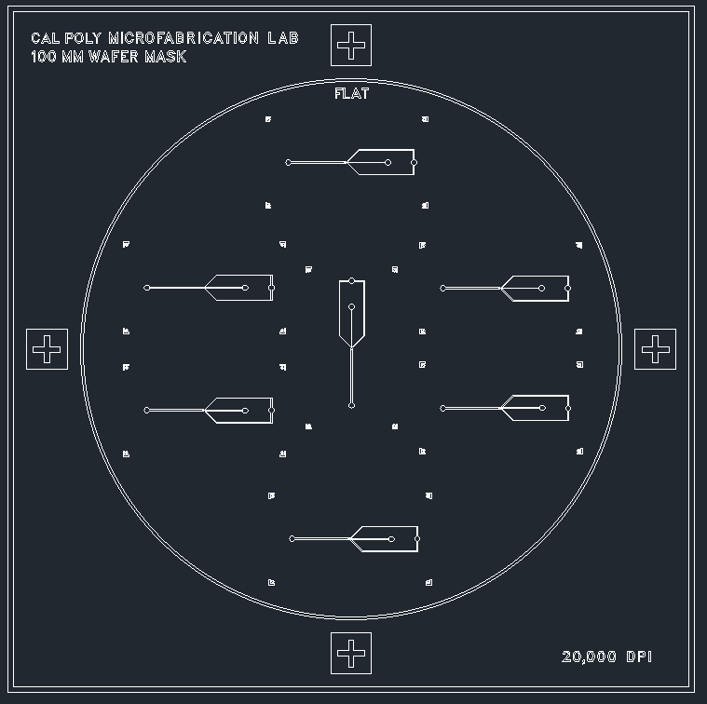
\includegraphics[width=0.6\textwidth]{images/micro_channel_mask.png}
    \caption{Micro channel mask by Josh Fadriquela \cite{fadriquela_design_2009-1}}
    \label{fig:microchannel_mask}
\end{figure}

\section[Objectives]{Thesis Purpose and Objectives}